\PassOptionsToPackage{unicode=true}{hyperref} % options for packages loaded elsewhere
\PassOptionsToPackage{hyphens}{url}
%
\documentclass[ignorenonframetext,]{beamer}
\usepackage{pgfpages}
\setbeamertemplate{caption}[numbered]
\setbeamertemplate{caption label separator}{: }
\setbeamercolor{caption name}{fg=normal text.fg}
\beamertemplatenavigationsymbolsempty
% Prevent slide breaks in the middle of a paragraph:
\widowpenalties 1 10000
\raggedbottom
\setbeamertemplate{part page}{
\centering
\begin{beamercolorbox}[sep=16pt,center]{part title}
  \usebeamerfont{part title}\insertpart\par
\end{beamercolorbox}
}
\setbeamertemplate{section page}{
\centering
\begin{beamercolorbox}[sep=12pt,center]{part title}
  \usebeamerfont{section title}\insertsection\par
\end{beamercolorbox}
}
\setbeamertemplate{subsection page}{
\centering
\begin{beamercolorbox}[sep=8pt,center]{part title}
  \usebeamerfont{subsection title}\insertsubsection\par
\end{beamercolorbox}
}
\AtBeginPart{
  \frame{\partpage}
}
\AtBeginSection{
  \ifbibliography
  \else
    \frame{\sectionpage}
  \fi
}
\AtBeginSubsection{
  \frame{\subsectionpage}
}
\usepackage{lmodern}
\usepackage{amssymb,amsmath}
\usepackage{ifxetex,ifluatex}
\usepackage{fixltx2e} % provides \textsubscript
\ifnum 0\ifxetex 1\fi\ifluatex 1\fi=0 % if pdftex
  \usepackage[T1]{fontenc}
  \usepackage[utf8]{inputenc}
  \usepackage{textcomp} % provides euro and other symbols
\else % if luatex or xelatex
  \usepackage{unicode-math}
  \defaultfontfeatures{Ligatures=TeX,Scale=MatchLowercase}
\fi
% use upquote if available, for straight quotes in verbatim environments
\IfFileExists{upquote.sty}{\usepackage{upquote}}{}
% use microtype if available
\IfFileExists{microtype.sty}{%
\usepackage[]{microtype}
\UseMicrotypeSet[protrusion]{basicmath} % disable protrusion for tt fonts
}{}
\IfFileExists{parskip.sty}{%
\usepackage{parskip}
}{% else
\setlength{\parindent}{0pt}
\setlength{\parskip}{6pt plus 2pt minus 1pt}
}
\usepackage{hyperref}
\hypersetup{
            pdftitle={Activités de recherche - une présentation pour GAMBLE},
            pdfauthor={Alba Marina MÁLAGA SABOGAL},
            pdfborder={0 0 0},
            breaklinks=true}
\urlstyle{same}  % don't use monospace font for urls
\newif\ifbibliography
\usepackage{graphicx,grffile}
\makeatletter
\def\maxwidth{\ifdim\Gin@nat@width>\linewidth\linewidth\else\Gin@nat@width\fi}
\def\maxheight{\ifdim\Gin@nat@height>\textheight\textheight\else\Gin@nat@height\fi}
\makeatother
% Scale images if necessary, so that they will not overflow the page
% margins by default, and it is still possible to overwrite the defaults
% using explicit options in \includegraphics[width, height, ...]{}
\setkeys{Gin}{width=\maxwidth,height=\maxheight,keepaspectratio}
\setlength{\emergencystretch}{3em}  % prevent overfull lines
\providecommand{\tightlist}{%
  \setlength{\itemsep}{0pt}\setlength{\parskip}{0pt}}
\setcounter{secnumdepth}{0}

% set default figure placement to htbp
\makeatletter
\def\fps@figure{htbp}
\makeatother


\title{Activités de recherche - une présentation pour GAMBLE}
\author{Alba Marina MÁLAGA SABOGAL}
\date{14 mai 2020}

\begin{document}
\frame{\titlepage}

\hypertarget{systuxe8mes-dynamiques}{%
\section{Systèmes dynamiques}\label{systuxe8mes-dynamiques}}

\begin{frame}{Le problème général}
\protect\hypertarget{le-probluxe8me-guxe9nuxe9ral}{}

\begin{itemize}
\tightlist
\item
  Evolution deterministe à court terme, qu'on connaît.
\item
  Les questions qu'on se pose concernent l'évolution à long terme.
\end{itemize}

\end{frame}

\begin{frame}{Un exemple concret : les rotations du cercle:}
\protect\hypertarget{un-exemple-concret-les-rotations-du-cercle}{}

\(α\) nombre\\
\(ρ:𝕊^1\to 𝕊^1\) rotation par un angle \(α\)\\

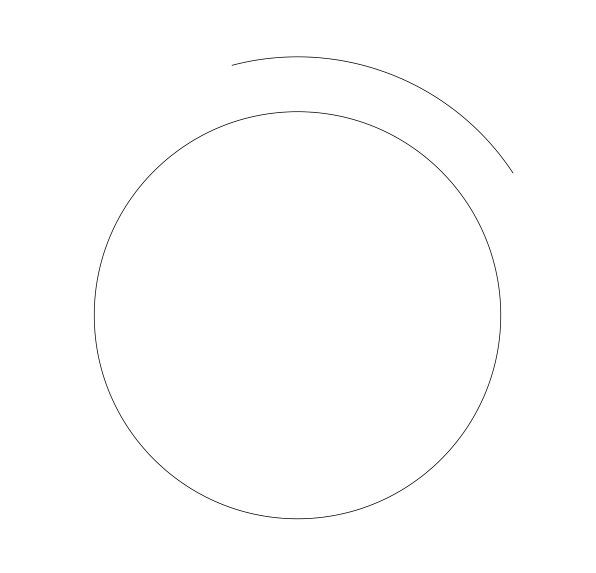
\includegraphics[width=\textwidth,height=3.125in]{cercle-arc.png}

Conjugué à :

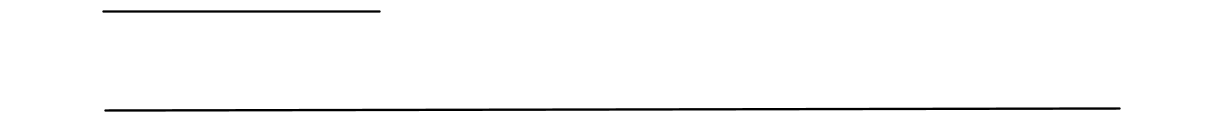
\includegraphics{segment-segment.png}

\(𝕋 = ℝ/ℤ = [0,1]/\{0~1\}\).

\end{frame}

\begin{frame}{Les rotations comme échanges d'intervalles}
\protect\hypertarget{les-rotations-comme-uxe9changes-dintervalles}{}

Paramétre: \(α ∈ [0,1[\)\\
Espace des phases: \(𝕋 = ℝ/ℤ = [0,1]/\{0~1\}\)\\

\(\begin{array}{rcrcl} ρ_- & : & [0,1-α[ & \to & [α,1[\\  & & x & \mapsto & x + α \end{array}\)

\(\begin{array}{rcrcl} ρ_+ & : & [1-α,1[ & \to & [0,α[\\  & & x & \mapsto & x + α - 1 \end{array}\)

\end{frame}

\begin{frame}{Un exemple fondamental: le tore}
\protect\hypertarget{un-exemple-fondamental-le-tore}{}

\href{http://albamath.com/snake}{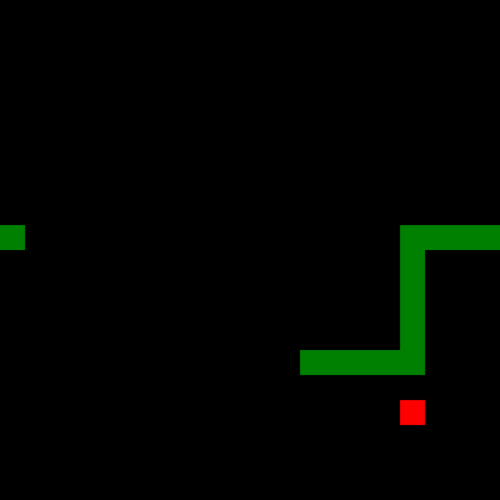
\includegraphics{snake-on-a-torus.png}}

\end{frame}

\begin{frame}{La caracteristique d'Euler et le genre:}
\protect\hypertarget{la-caracteristique-deuler-et-le-genre}{}

\href{http://albamath.com/snake}{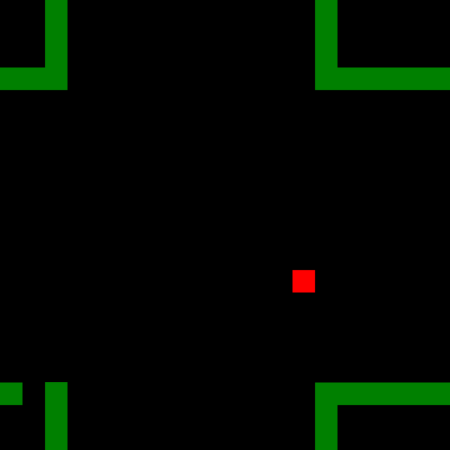
\includegraphics{snake-around-corners.png}}

\(χ = V-E+F = 1 - 2 + 1 = 0\)\\
\(χ=2-2g\)\\
\(g=1\)

\end{frame}

\begin{frame}{Un autre exemple simple de surface de translation: le L}
\protect\hypertarget{un-autre-exemple-simple-de-surface-de-translation-le-l}{}

\href{http://albamath.com/snake-L}{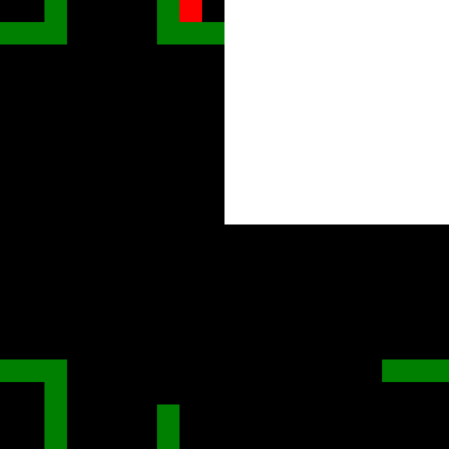
\includegraphics{snake-l-corner.png}}

\end{frame}

\begin{frame}{La caracteristique d'Euler et le genre du L:}
\protect\hypertarget{la-caracteristique-deuler-et-le-genre-du-l}{}

\href{http://albamath.com/snake-L}{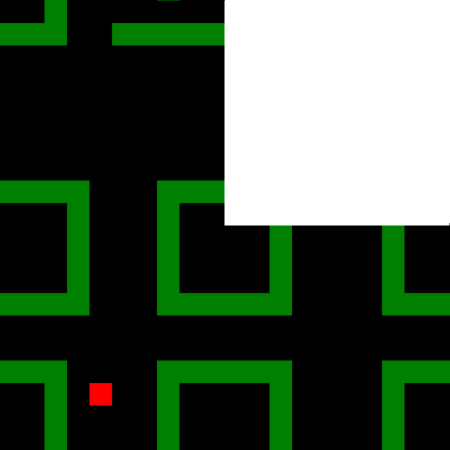
\includegraphics{snake-l-corner-4.png}}

\(χ = V-E+F = 1 - 2 + 1 = 0\)\\
\(χ=2-2g\)\\
\(g=1\)

\end{frame}

\begin{frame}{Une autre vue du L:}
\protect\hypertarget{une-autre-vue-du-l}{}

\href{http://albamath.com/snakeX}{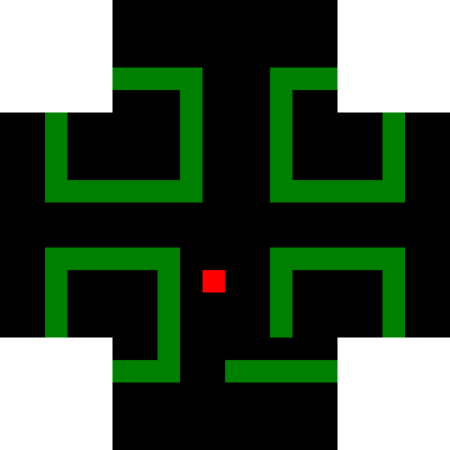
\includegraphics{snake-x-corner-4.png}}

\(χ = V-E+F = 1 - 6 + 3 = -2\)\\
\(χ=2-2g\)\\
\(g=2\)

\end{frame}

\begin{frame}{Définition de surface de translation ``finie''.}
\protect\hypertarget{duxe9finition-de-surface-de-translation-finie.}{}

Une surface de translation est une surface compacte sans bord qui,
privée d'un nombre fini de points, possède un atlas tel que que les
changements de cartes dans cet atlas sont des translations. Supposons
que l'atlas est maximal - les points non couverts par l'atlas sont des
singularités coniques de la géométrie de la surface avec un angle qui
est un multiple entier de 360 degrés.

\end{frame}

\begin{frame}{Dynamique sur une surface de translation}
\protect\hypertarget{dynamique-sur-une-surface-de-translation}{}

\begin{figure}
\centering

\includegraphics{flot-tore.tiff}
\caption{Dynamique sur le tore}
\end{figure}

\end{frame}

\begin{frame}{Billards: un contexte où les surfaces de translation
apparaissent naturellement}
\protect\hypertarget{billards-un-contexte-ouxf9-les-surfaces-de-translation-apparaissent-naturellement}{}

\begin{figure}
\centering

\includegraphics{rebond-carre.tiff}
\caption{rebond-carre.tiff}
\end{figure}

\end{frame}

\begin{frame}

\begin{figure}
\centering

\includegraphics{rebond-carre.tiff}
\caption{rebond-carre.tiff}
\end{figure}

\end{frame}

\begin{frame}

\begin{figure}
\centering

\includegraphics{depliage-2.tiff}
\caption{Commence à se deplier}
\end{figure}

\end{frame}

\begin{frame}

\begin{figure}
\centering

\includegraphics{flot-L.tiff}
\caption{Continue}
\end{figure}

\end{frame}

\begin{frame}

\begin{figure}
\centering

\includegraphics{flot-tore.tiff}
\caption{On obtient le flot sur le tore}
\end{figure}

\end{frame}

\begin{frame}{Questions ouvertes sur des billards polygonaux:}
\protect\hypertarget{questions-ouvertes-sur-des-billards-polygonaux}{}

\begin{itemize}
\tightlist
\item
  il existe toujours des trajectoires périodiques ?
\item
  toutes les trajectoires sont denses ? (\textbf{minimalité})
\item
  il y a ou pas des partitions non triviales (en mesure) en
  sous-ensembles invariants ? (\textbf{ergodicité})
\end{itemize}

\begin{figure}
\centering
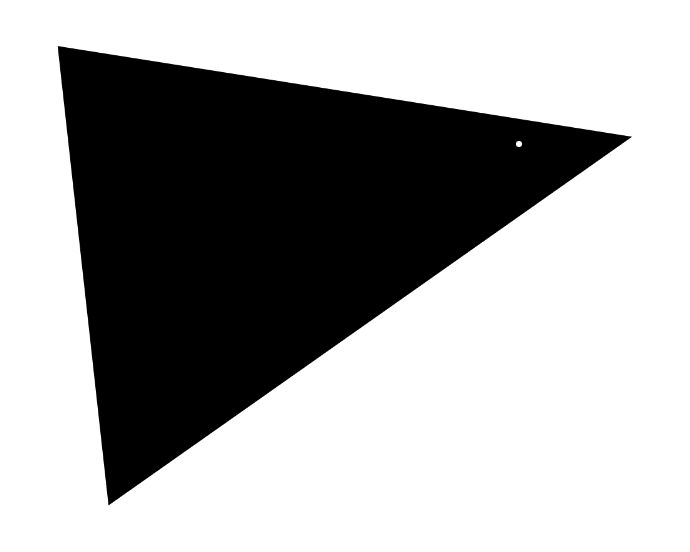
\includegraphics{triangle-1.png}
\caption{triangle-1.png}
\end{figure}

La troisième question de cette liste était le point de départ de ma
thèse, effectuée de 2011 à 2014 à Orsay sous la direction de
Jean-Christophe Yoccoz. La question est encore ouverte, he he, c'est à
dire que finalement dans ma thèse je réponds à d'autres questions
(moralement) en rapport avec celle-ci.

\end{frame}

\begin{frame}{Cylindres discrets - motivation}
\protect\hypertarget{cylindres-discrets---motivation}{}

\begin{figure}
\centering
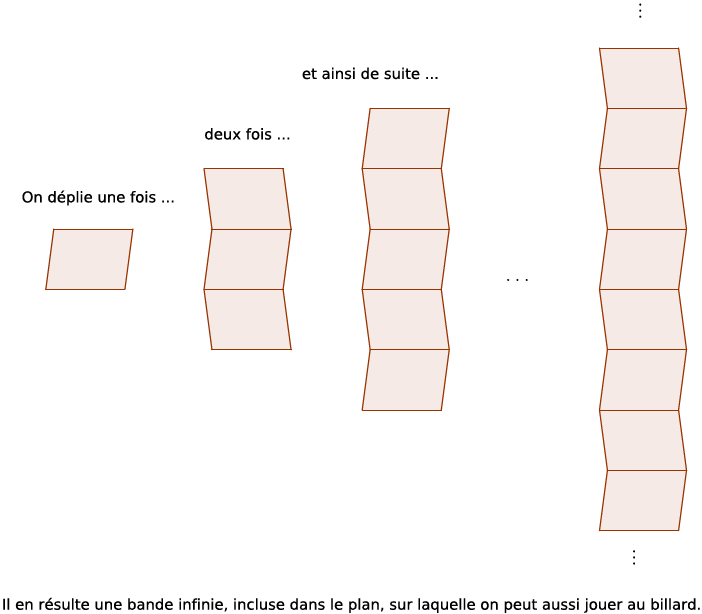
\includegraphics{parallelogramme-deplie-n-fois.png}
\caption{Parallélogramme deplié partiellement}
\end{figure}

\end{frame}

\begin{frame}

\begin{figure}
\centering

\includegraphics{rebond-cas-special.tiff}
\caption{rebond-cas-special.tiff}
\end{figure}

Similarité avec des familles d'applications sur le cylindre discret
\(ℤ×𝕋\). L'étude de la dynamique de ces applications fût finalement
l'objet de ma thèse.

\end{frame}

\begin{frame}{Une famille de transformations du cylindre discret
\(ℤ×𝕋\)}
\protect\hypertarget{une-famille-de-transformations-du-cylindre-discret-ux2124ux1d54b}{}

Considérons une suite bi-infinie de paramètres de rotation
\(α_n∈𝕋 = [0,1]/\{0~1\}\). Pour chaque suite de la sorte, appliquons la
rotation par \(α_n\) au cercle \(\{n\}×𝕋\). Puis, coupons tous les
cercles en deux intervalles de même longueur, independants des
paramètres de rotation, et considérons leur intérieur, qu'on appelera la
partie descendante, et la partie montante, puis déplaçons la partie de
droite de un niveau vers le haut et la partie de gauche d'un niveau vers
le bàs.

Ainsi, à chaque suite bi-infinie \((α_n)_{n∈ℤ}\) correspond une
transformation du cylindre discret \(ℤ×𝕋\), définie partout sauf sur un
ensemble discret de points singuliers ( ceux qui après rotation
arriveraient sur les bords des parties montantes et descendants). C'est
cette famille de transformations \(T_{α_}\) que j'ai étudié dans ma
thèse.

\end{frame}

\begin{frame}{Dynamique générique d'une famille de transformations de
\(ℤ×𝕋\)}
\protect\hypertarget{dynamique-guxe9nuxe9rique-dune-famille-de-transformations-de-ux2124ux1d54b}{}

Espace de paramètres \(𝕋^n\), dispose d'une mesure de probabilité et
d'une topologie produit.

Pour simplifier les notations, on va écrire \(α\) pour la suite
\((α_n)_{n\in ℤ}\). Dans ma thèse j'ai demontré que:

\begin{itemize}
\tightlist
\item
  presque sùrement, \(T_α\) n'a pas d'ensemble errant de mesure positive
\item
  génériquement: - \(T_α\) est conservative - toute demi-orbite \(T_α\)
  définie pour une infinité d'itérations est dense (c-à-d \(T_α\) est
  \textbf{minimal}) - tout sous-ensemble invariant par \(T_α\) est de
  mesure nulle ou bien a un complement de mesure nulle (c-à-d \(T_α\)
  est \textbf{ergodique})
\end{itemize}

\end{frame}

\begin{frame}{Techniques developpées dans la thèse}
\protect\hypertarget{techniques-developpuxe9es-dans-la-thuxe8se}{}

Pour montrer ces résultats, je me suis appuyé sur des résultats bien
connus pour des échanges d'intervalles, pour lesquelles les propriétés
dynamiques que j'étudiais était déjà bien connues:

\textbf{Thm (Poincaré)} Tout système dynamique de mesure finie est
conservatif.

\textbf{Thm (Keane)} Tout échange d'intervalles ``irréductible'' est
minimal.

\textbf{Thm (Masur-Tabachnikov)} Tout échange d'intervalle minimal est
aussi ergodique.

Ensuite, j'ai procédé par perturbations: des valeurs spéciales de
\(α_n=±½\), (c-à-d les rotations par un demi-tour), permettent d'obtenir
des sous-ensembles dans l'espace des phases qui sont invariants et qui
sont des échanges d'intervalles classiques. Ensuite, en traduit la
propriété dynamique qu'on veut montrer dans une formule quantitative et
puis on construit des ouverts denses autour de ces paramètres spéciaux
en prenant garde à ne pertuber qu'un petit peu cette formule.

\end{frame}

\begin{frame}{Les surfaces en escalier.}
\protect\hypertarget{les-surfaces-en-escalier.}{}

\begin{figure}
\centering

\includegraphics{escalier-infini.tiff}
\caption{Escalier regulier}
\end{figure}

\end{frame}

\begin{frame}{Le modèle wind-tree des Ehrenfest:}
\protect\hypertarget{le-moduxe8le-wind-tree-des-ehrenfest}{}

\href{https://rantonse.no/demos/MirrorRoom/}{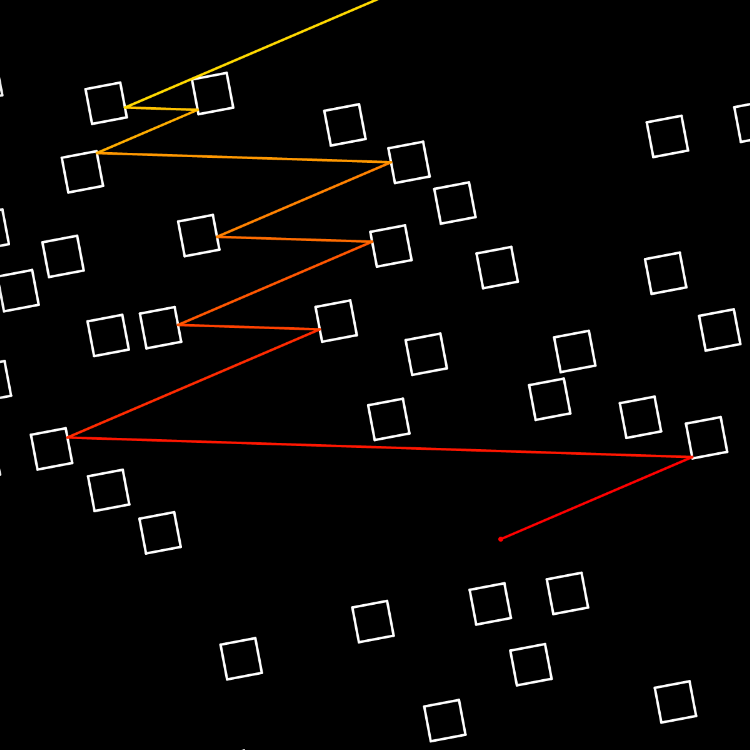
\includegraphics{wind-tree.png}}

Avec Serge Troubetzkoy, on a montré que génériquement, la dynamique du
wind-tree est minimale (2015), ergodique (2016), de puissances
cartésiennes ergodiques (2016-2017) et uniquement ergodique (2017-2019)
dans presque toute direction.

\end{frame}

\begin{frame}{Retour aux surfaces en escalier:}
\protect\hypertarget{retour-aux-surfaces-en-escalier}{}

\begin{figure}
\centering
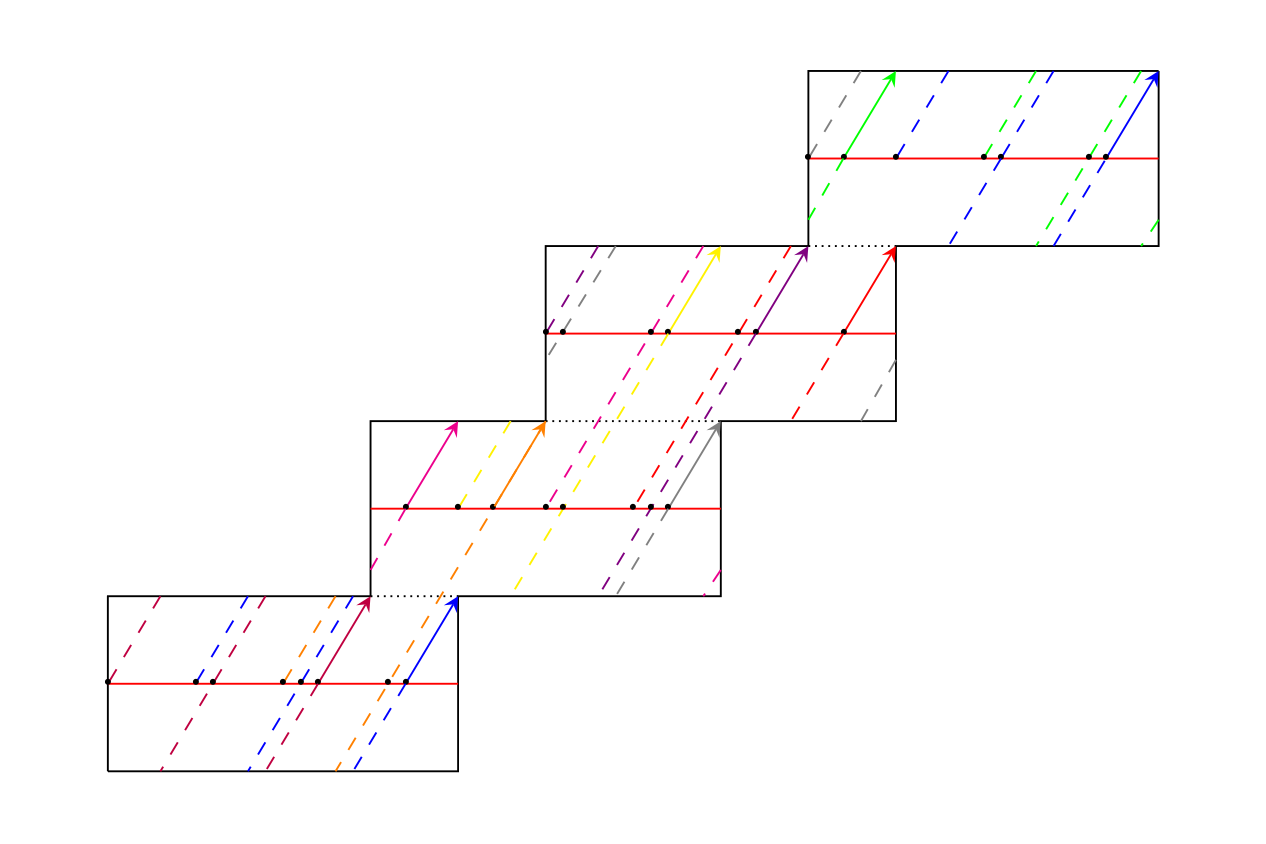
\includegraphics{orbites-escalier.png}
\caption{Orbites sur une surface en escalier à recouvrement variable}
\end{figure}

\end{frame}

\hypertarget{illustrations-des-mathuxe9matiques-et-intuxe9gration-dans-gamble}{%
\section{Illustrations des mathématiques et intégration dans
Gamble}\label{illustrations-des-mathuxe9matiques-et-intuxe9gration-dans-gamble}}

\begin{frame}{Tores plats et autres surfaces de translation pliées en
origami}
\protect\hypertarget{tores-plats-et-autres-surfaces-de-translation-pliuxe9es-en-origami}{}

\href{https://p3d.in/u/albamath/zJFfh}{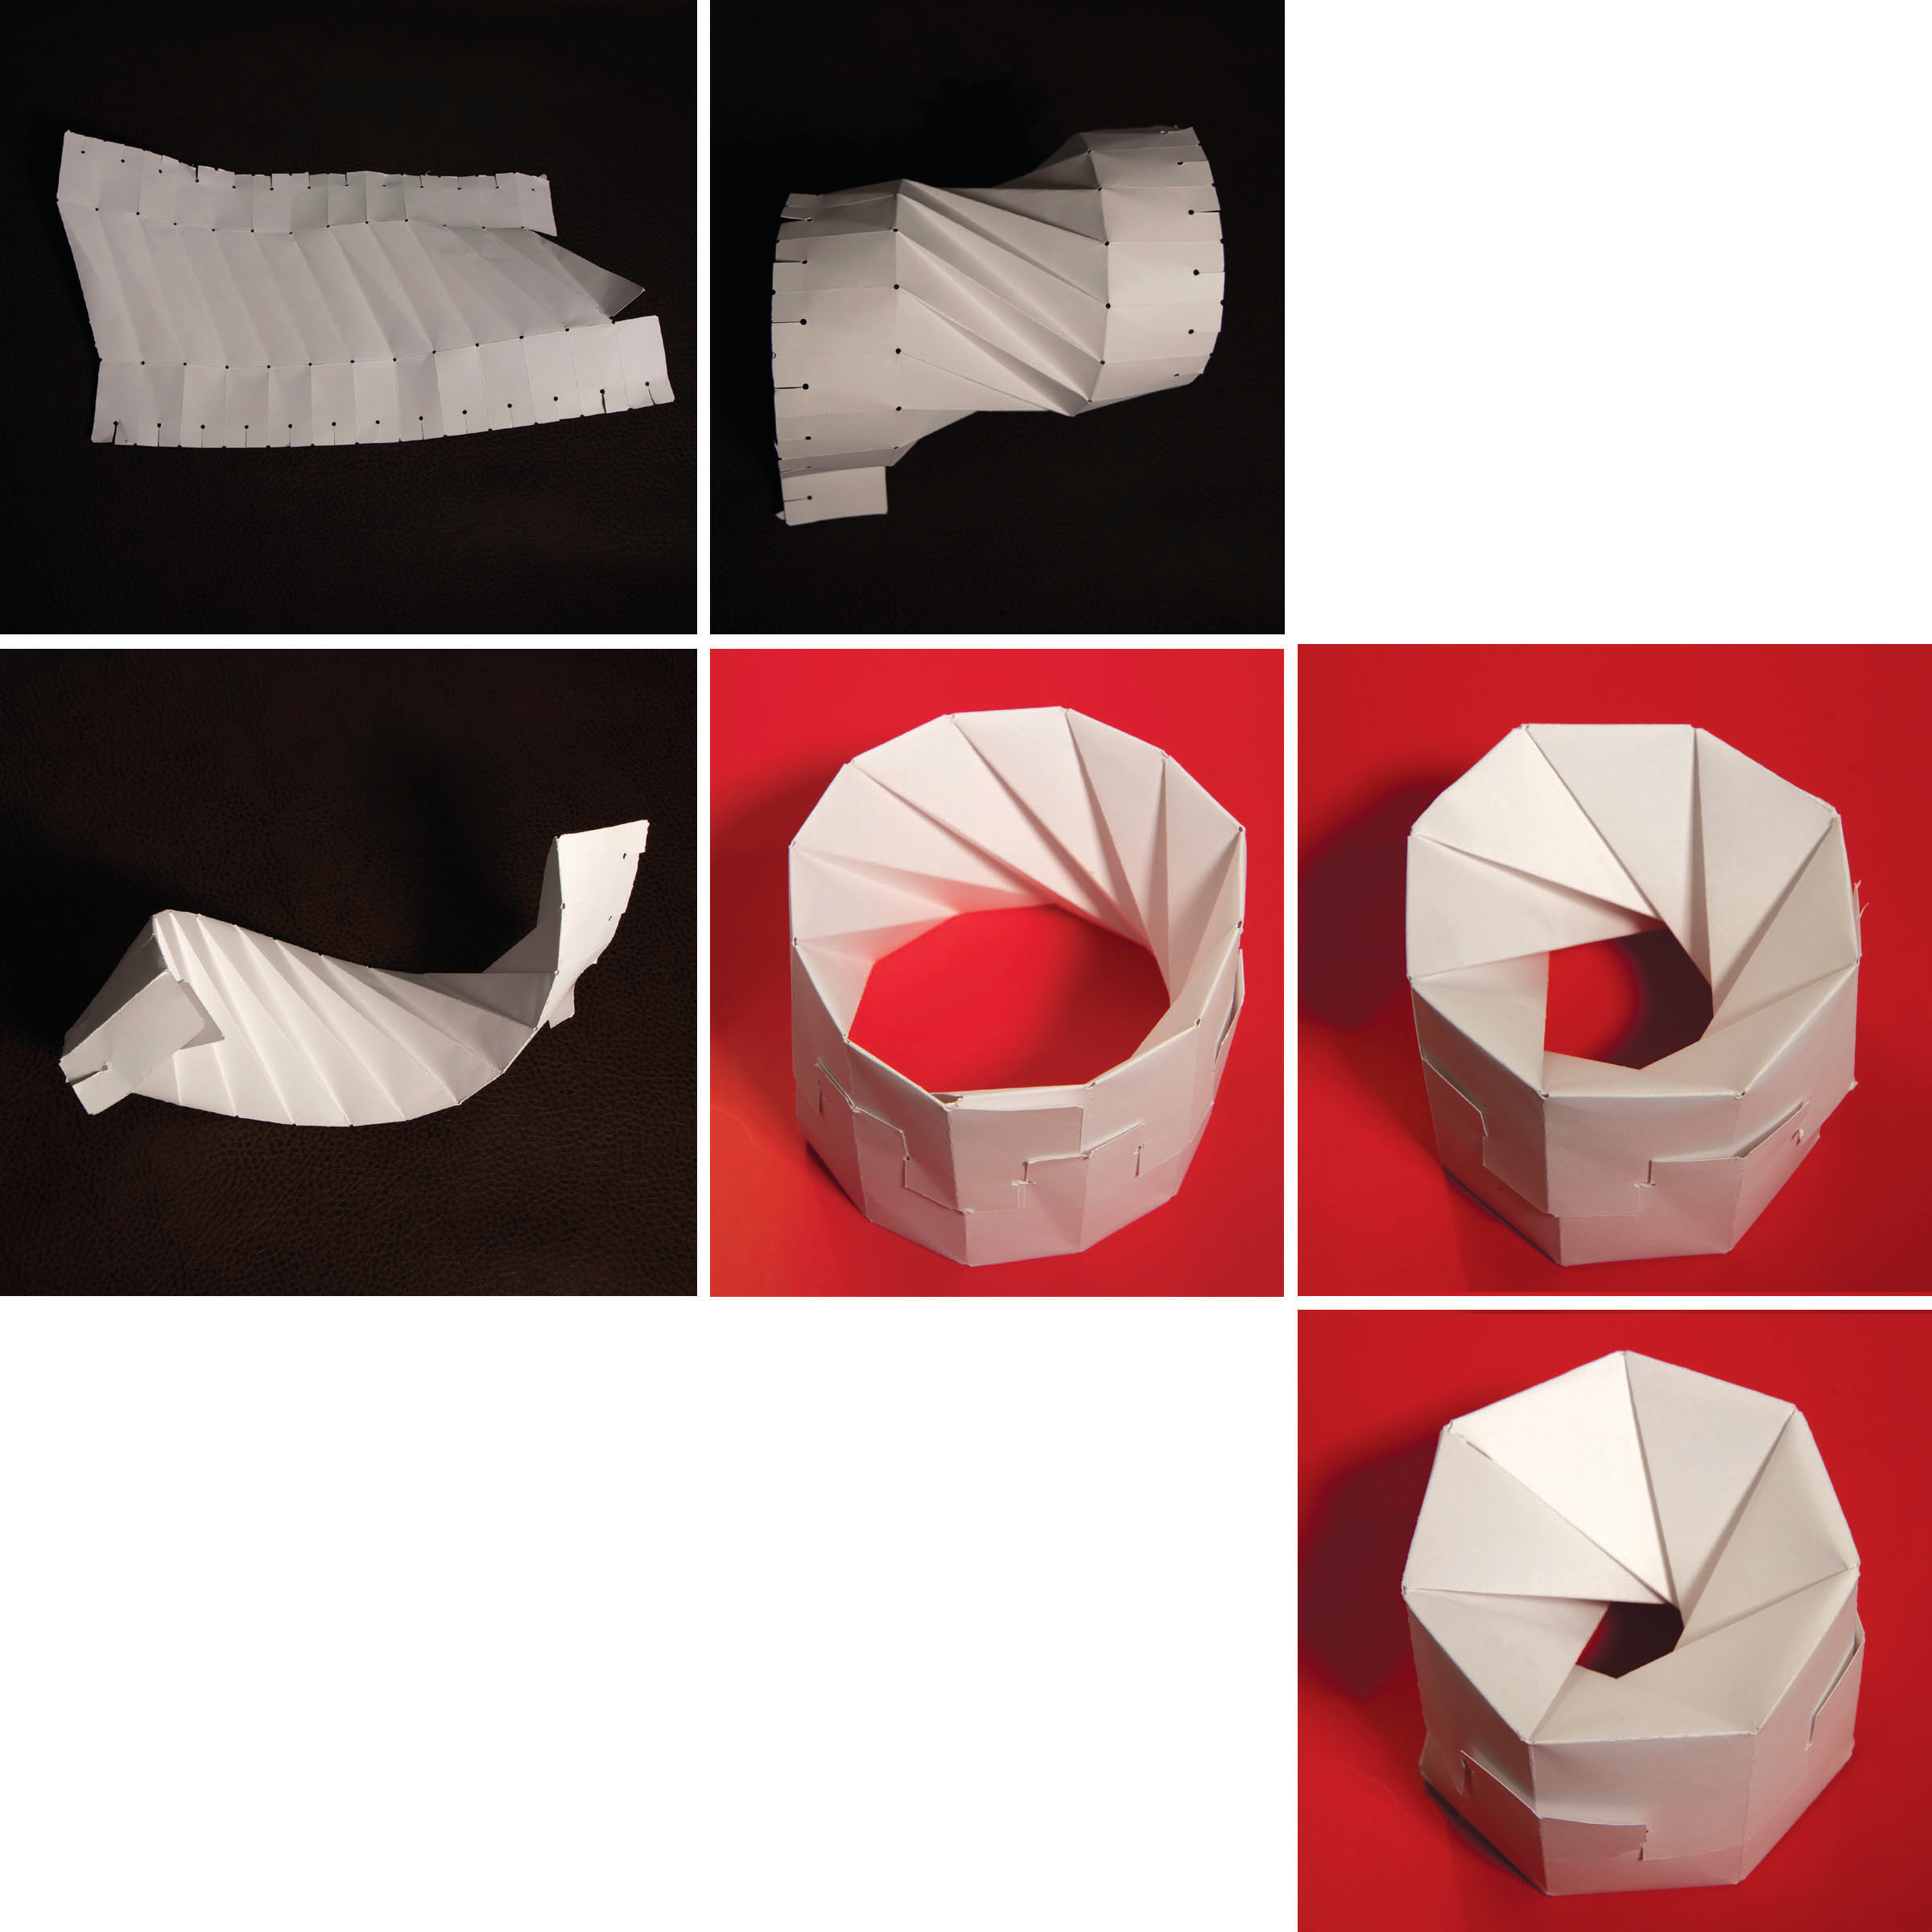
\includegraphics{flat-tori-harris.jpg}}

\end{frame}

\begin{frame}{Pliages en papier hyperbolique (ou Kombucha)}
\protect\hypertarget{pliages-en-papier-hyperbolique-ou-kombucha}{}

\begin{figure}
\centering
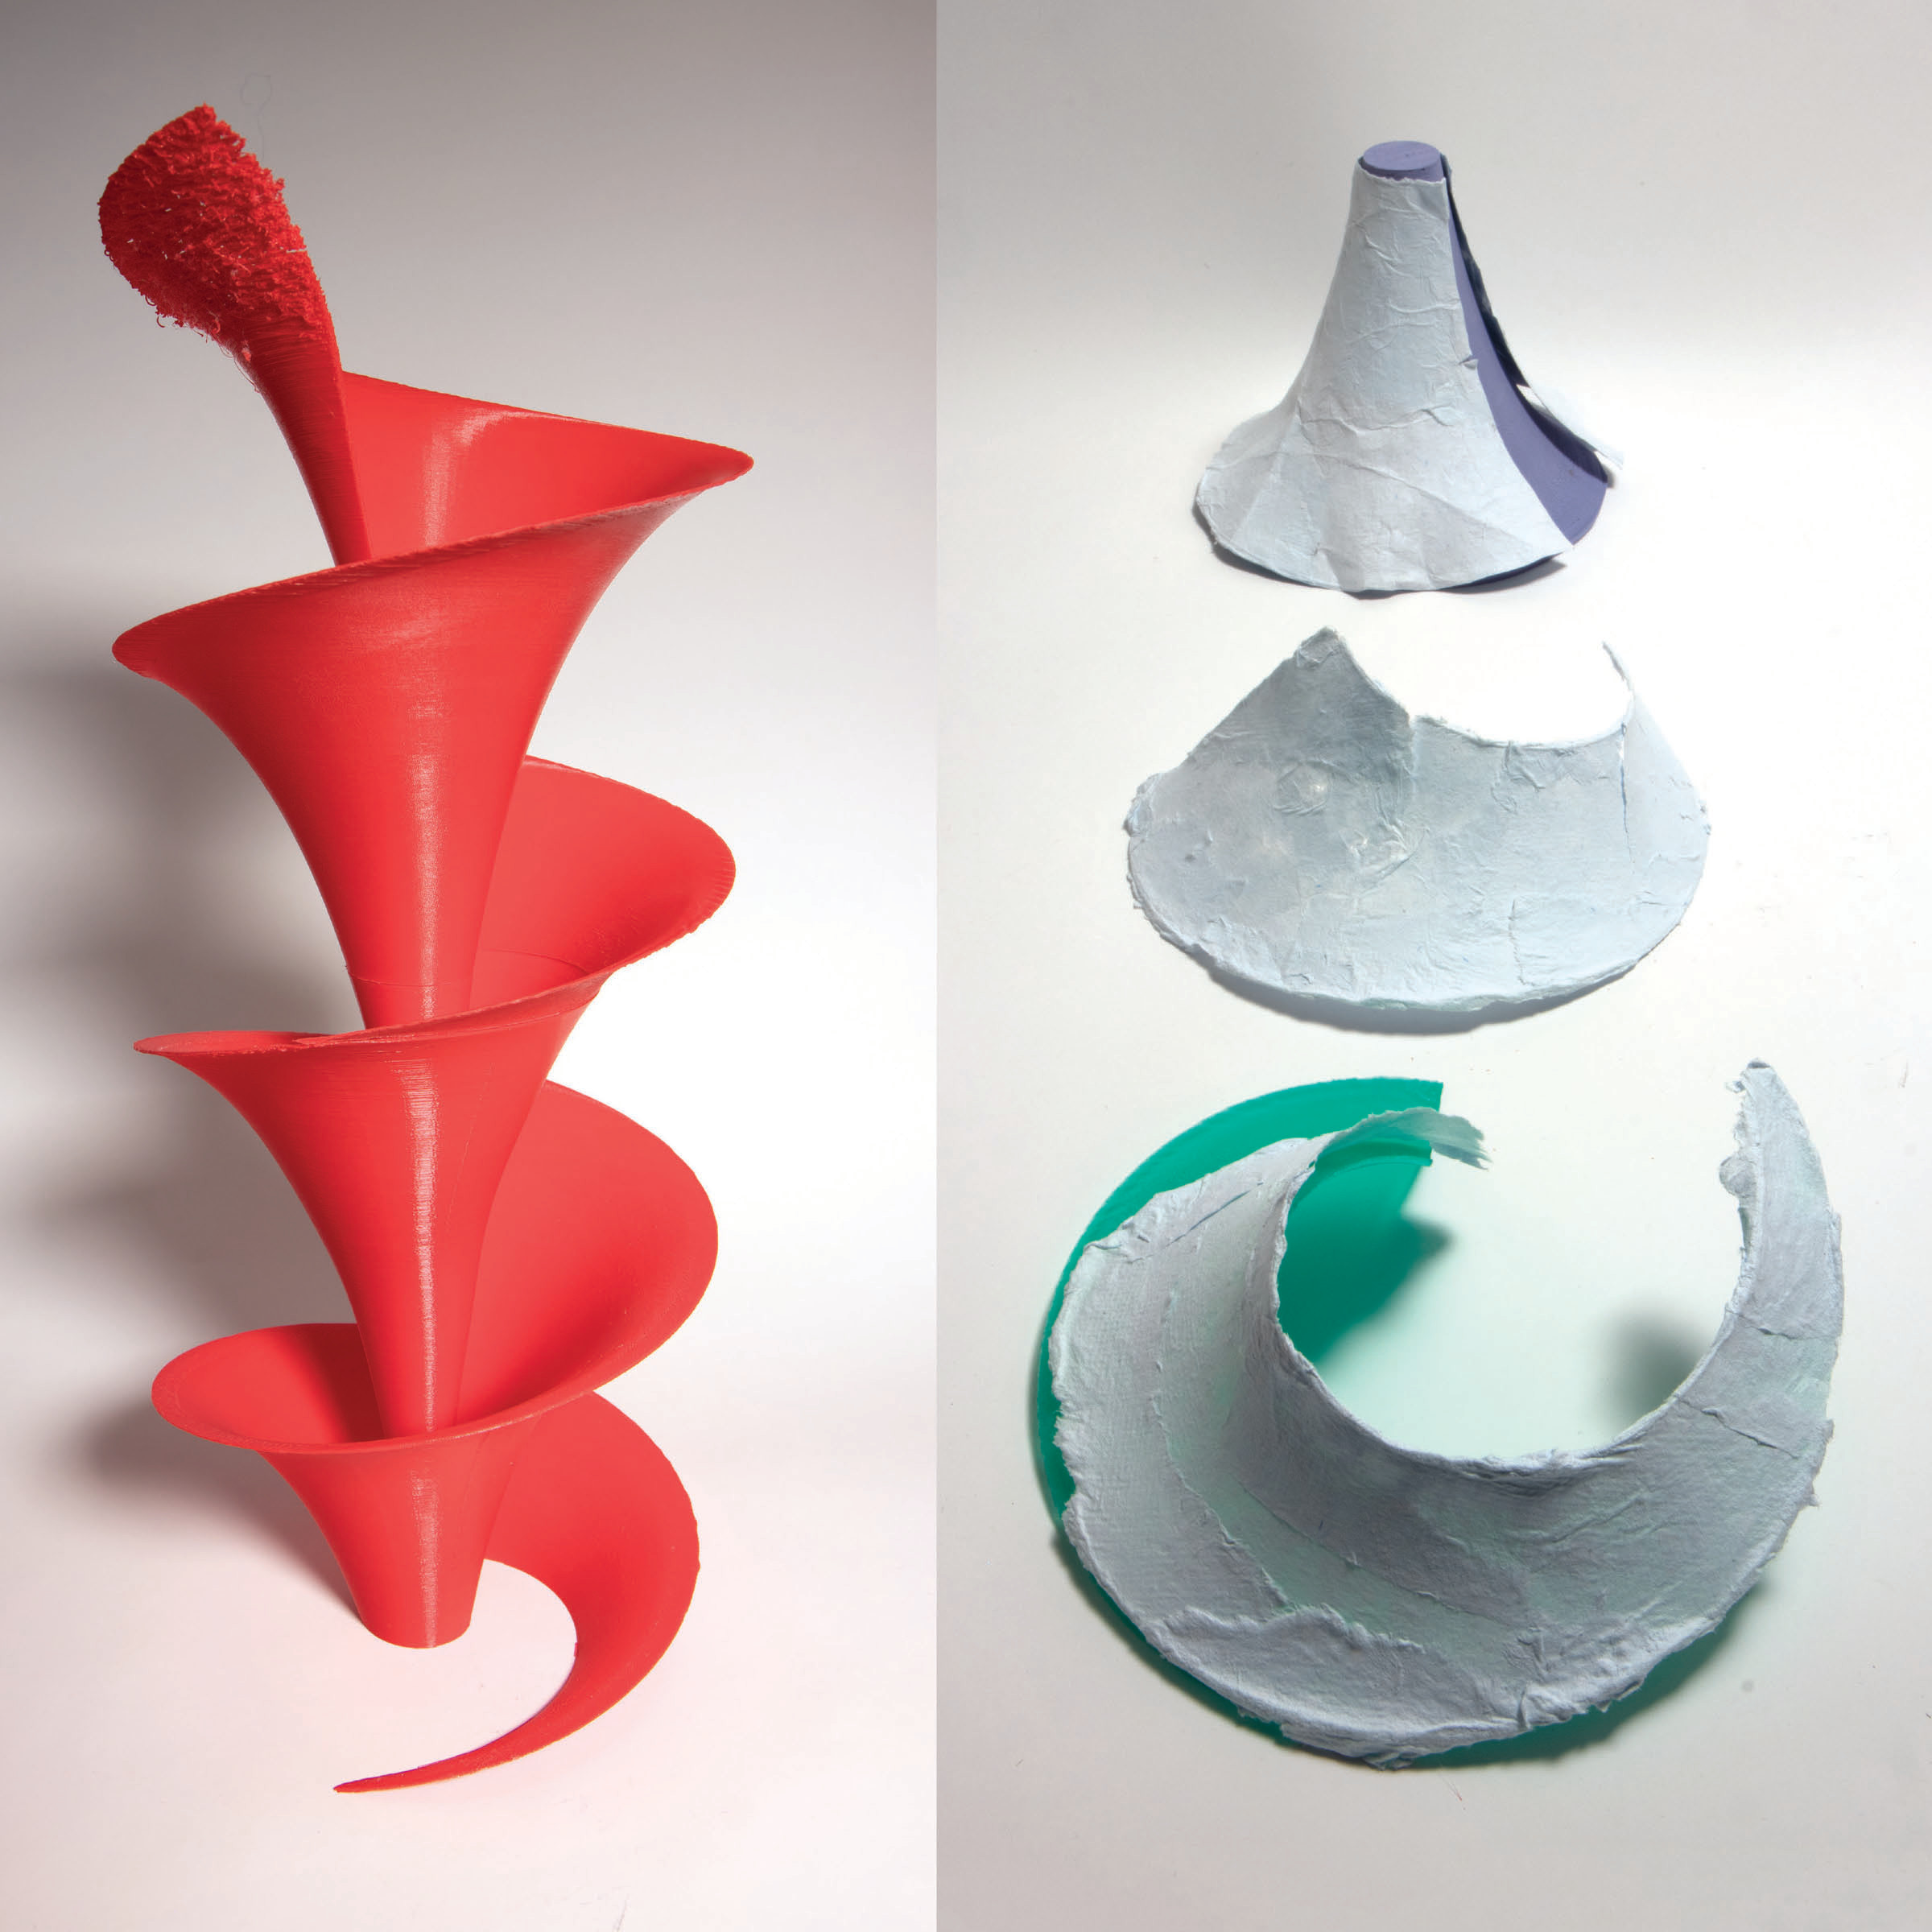
\includegraphics{hyperbolic-paper-harris.jpg}
\caption{Hyperbolic paper from Abrams, Paul, and me.}
\end{figure}

\end{frame}

\begin{frame}{Impression 3D de surfaces algébriques}
\protect\hypertarget{impression-3d-de-surfaces-alguxe9briques}{}

\begin{figure}
\centering
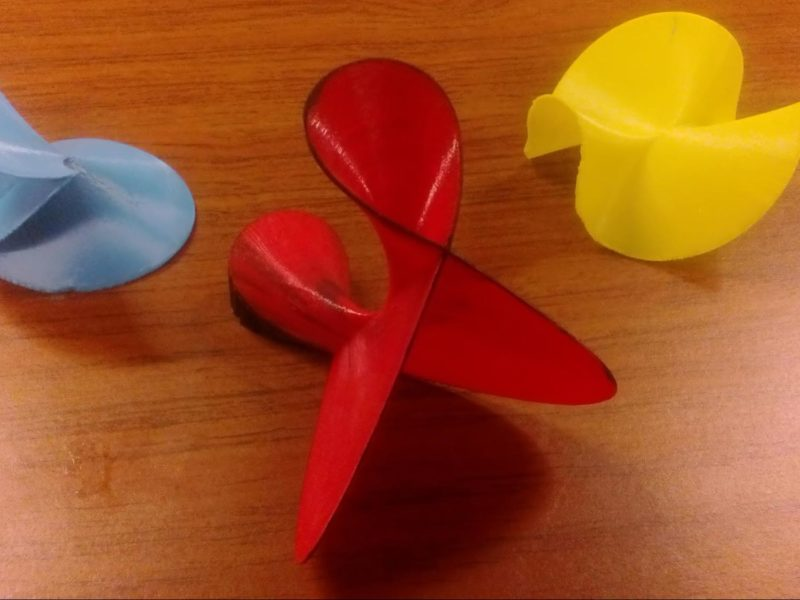
\includegraphics{surfaces-alg.jpg}
\caption{Quelques surfaces algébriques}
\end{figure}

\end{frame}

\begin{frame}

\begin{figure}
\centering
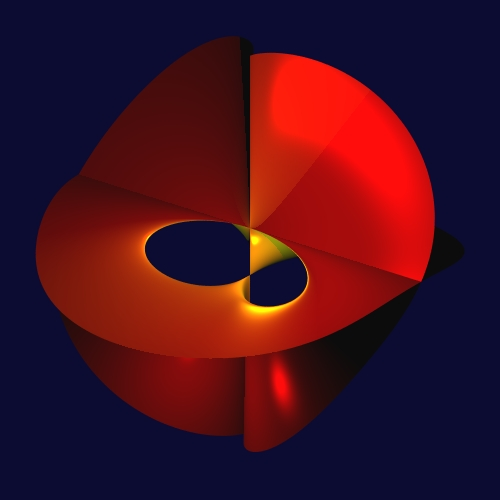
\includegraphics{miau.jpg}
\caption{Miaou par Herwig Hauser}
\end{figure}

\end{frame}

\begin{frame}{Impression 3D d'autres objets mathématiques}
\protect\hypertarget{impression-3d-dautres-objets-mathuxe9matiques}{}

\begin{figure}
\centering
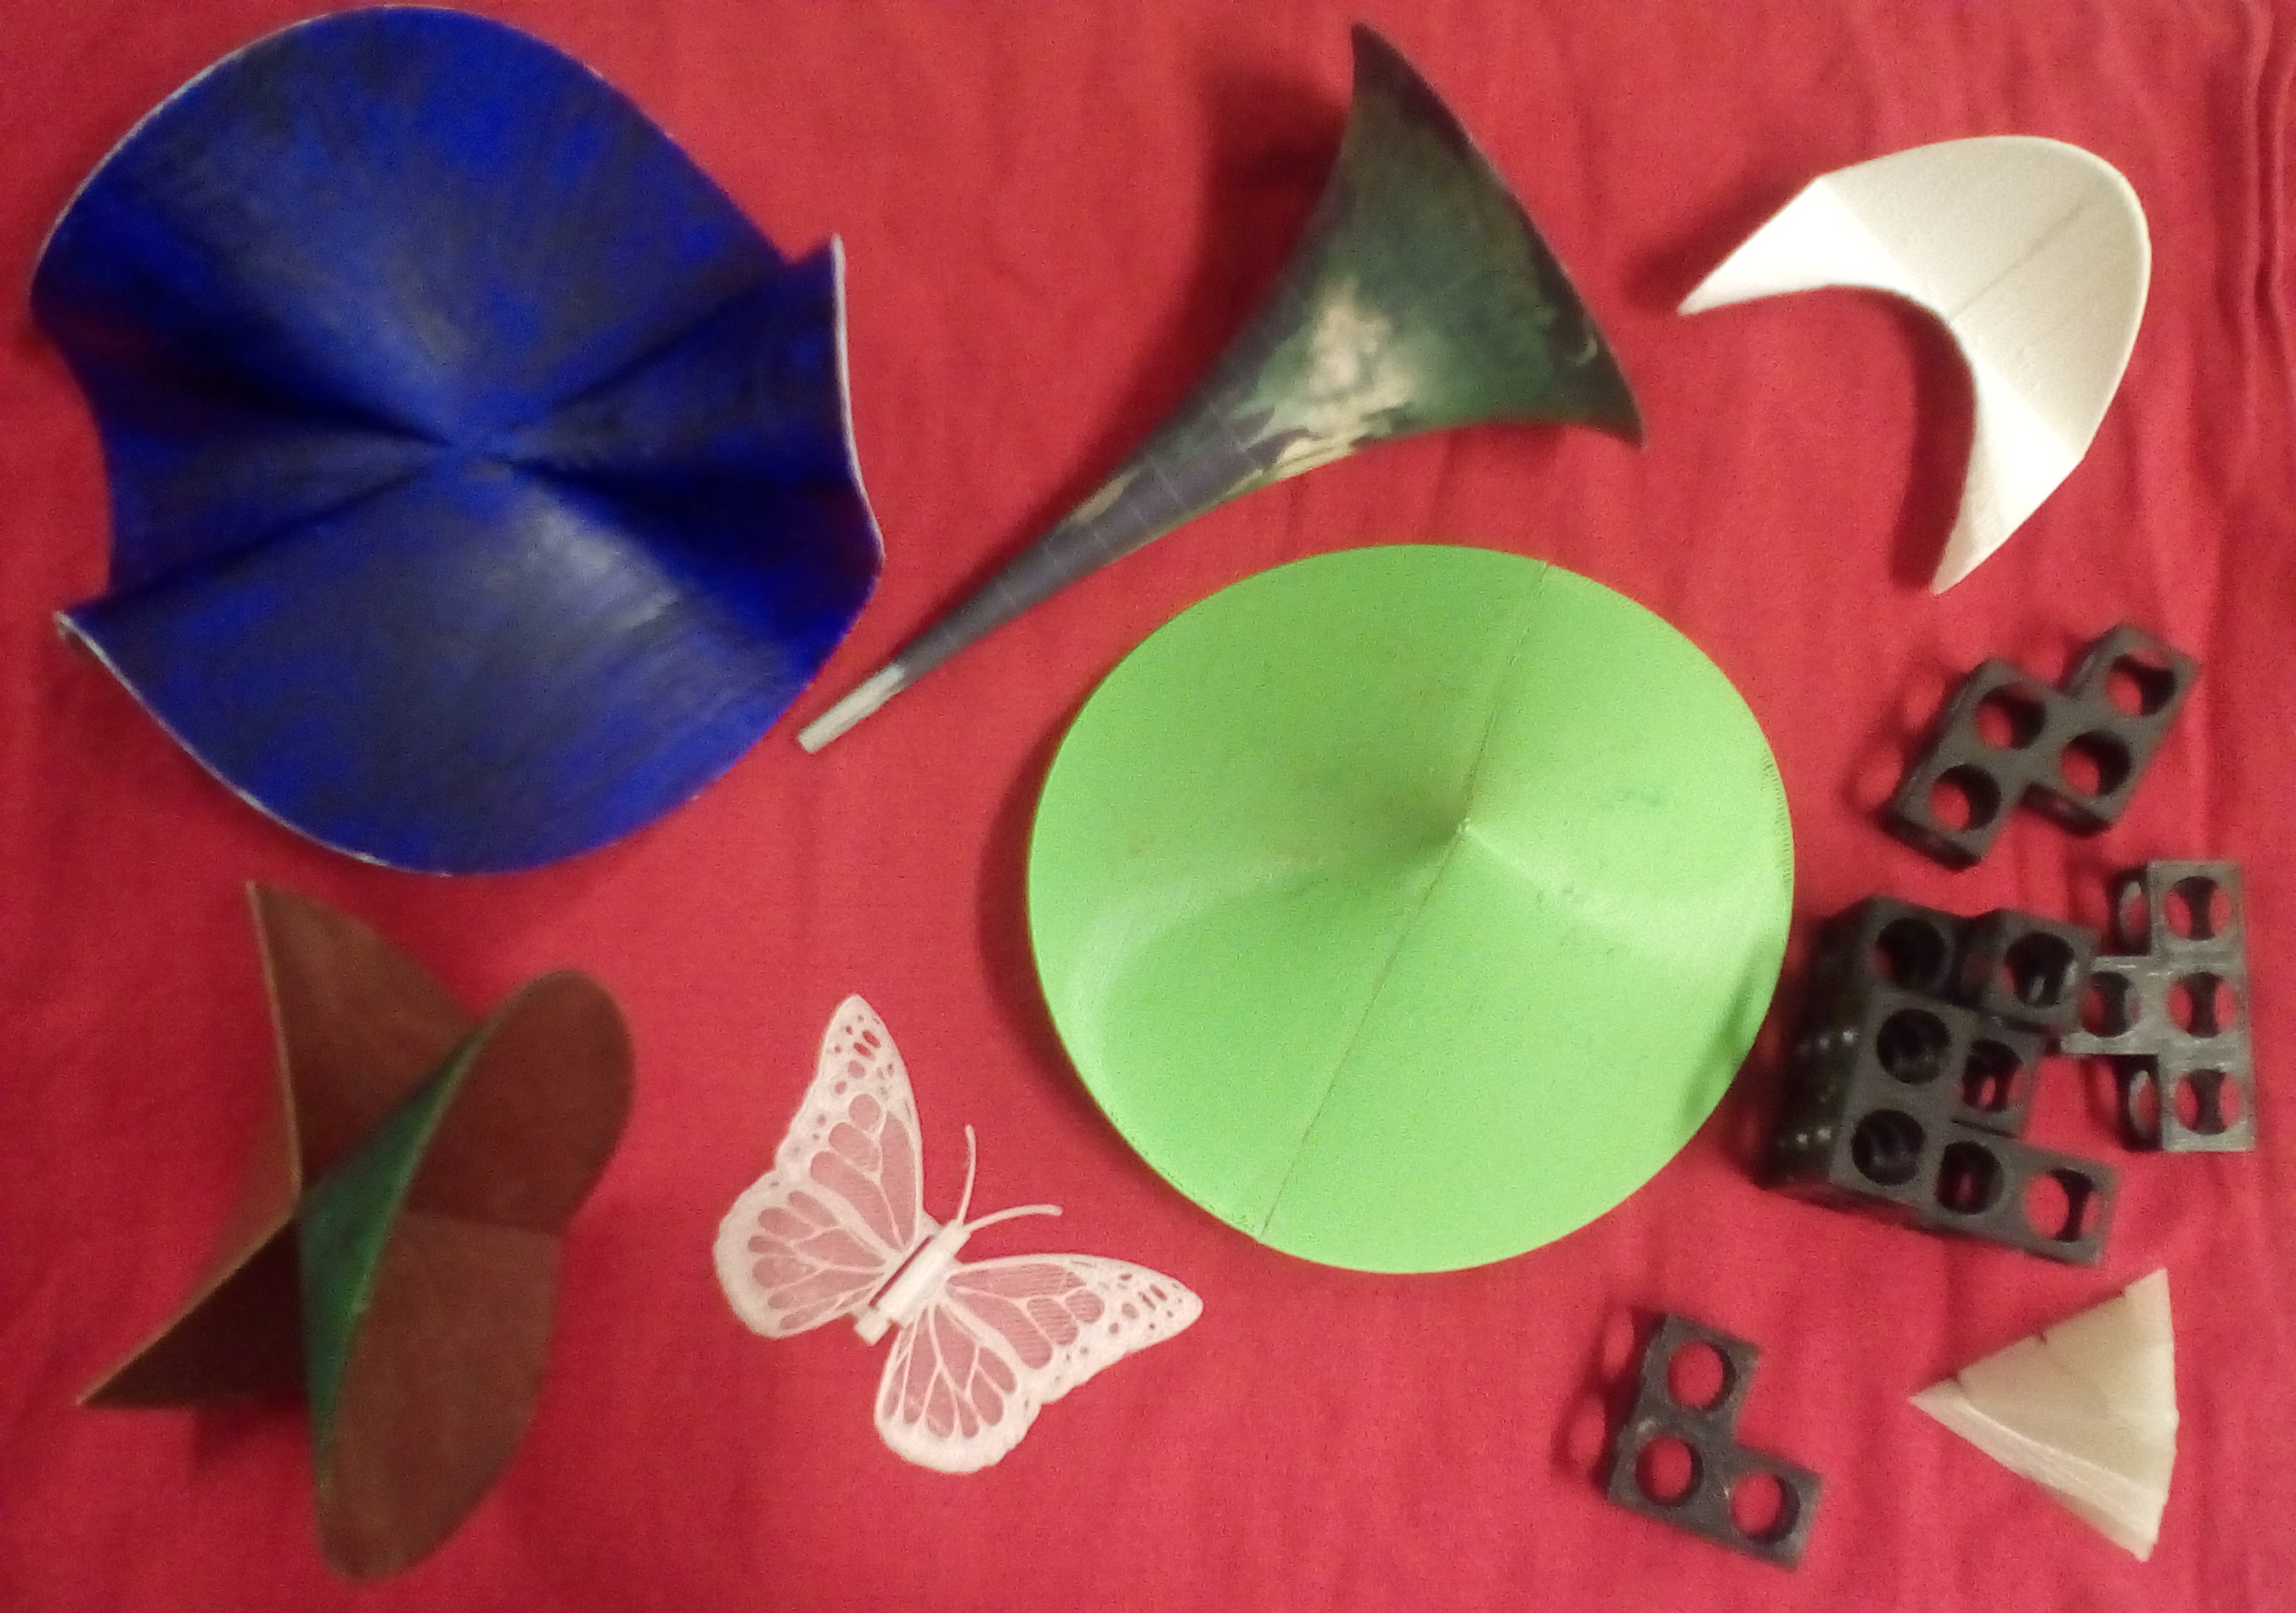
\includegraphics{objets-3D-sur-echarpe-rouge.png}
\caption{objets-3D-sur-echarpe-rouge.png}
\end{figure}

\end{frame}

\begin{frame}{Analyse d'anciens objets en plâtre}
\protect\hypertarget{analyse-danciens-objets-en-pluxe2tre}{}

\begin{figure}
\centering
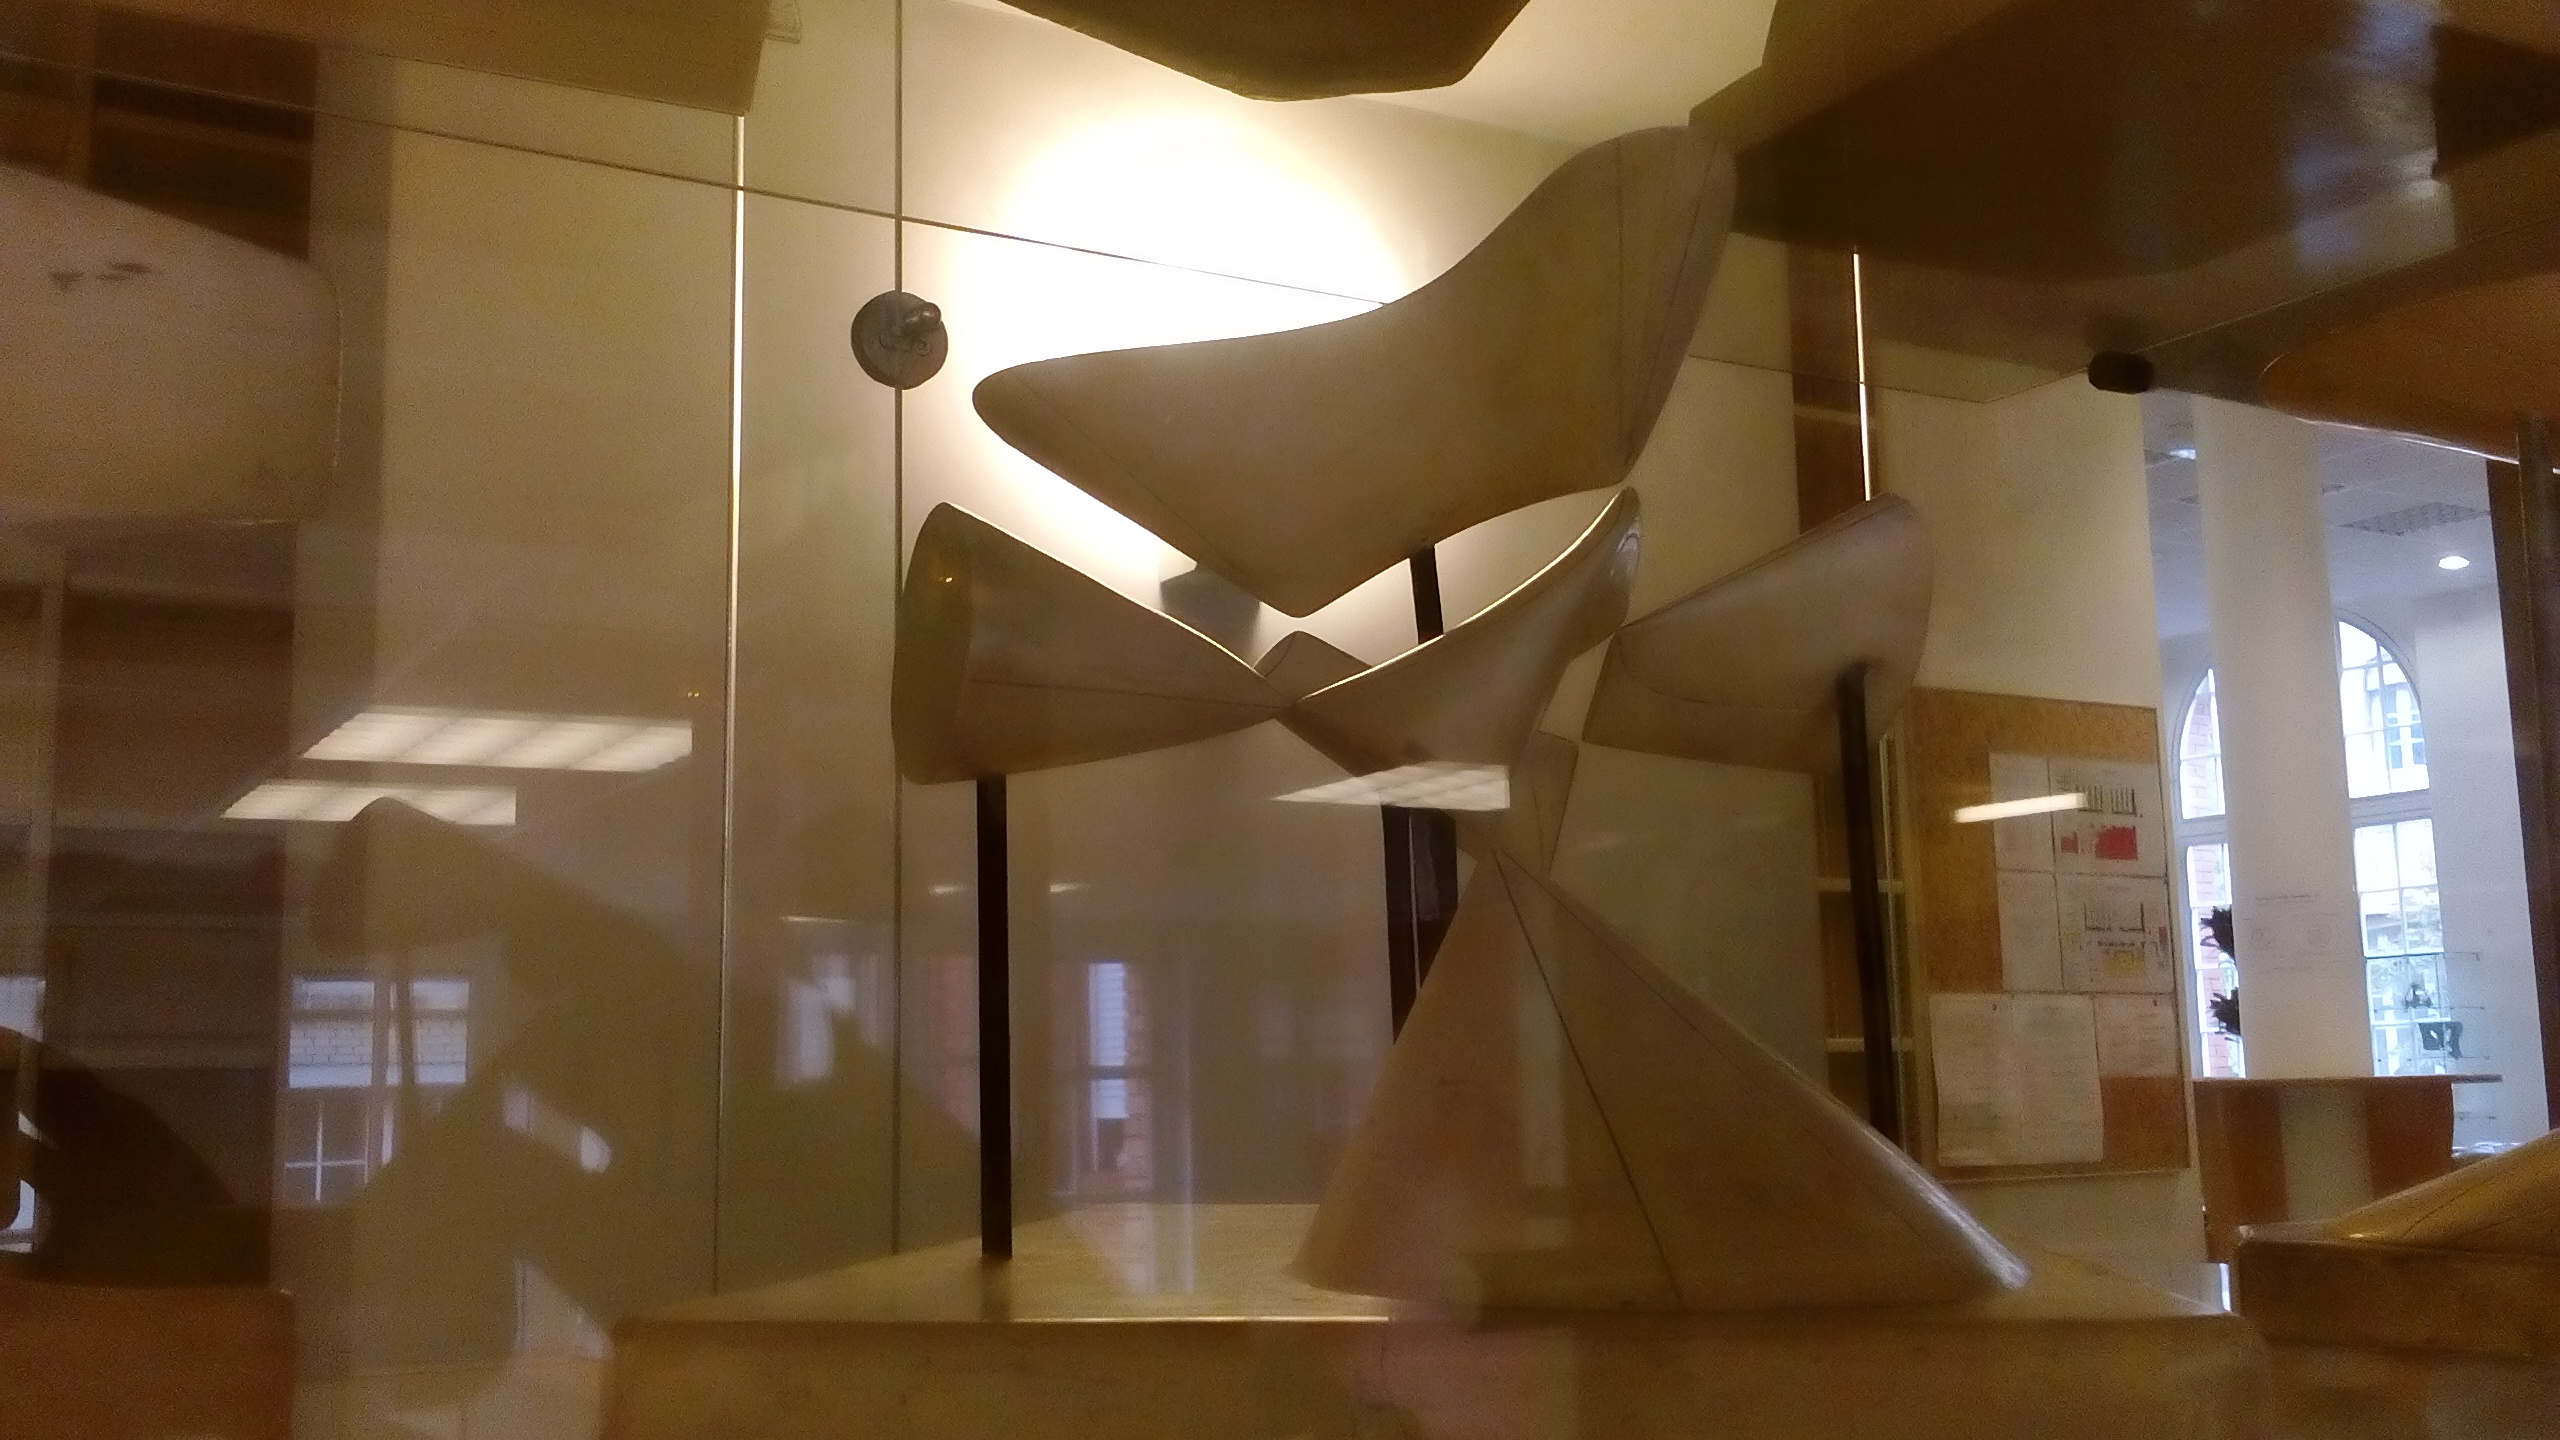
\includegraphics{kummer-platre-a.jpg}
\caption{Surface de Kummer, collections de l'IHP}
\end{figure}

\end{frame}

\hypertarget{ce-que-je-pense-que-je-peut-apporter-dans-gamble}{%
\section{Ce que (je pense que) je peut apporter dans
Gamble}\label{ce-que-je-pense-que-je-peut-apporter-dans-gamble}}

\begin{frame}{En tant que mathématicienne}
\protect\hypertarget{en-tant-que-mathuxe9maticienne}{}

Compétences poussées en:

\begin{itemize}
\tightlist
\item
  géométries 2D et 3D (y compris non-euclidiennes)
\item
  systèmes dynamiques
\end{itemize}

Compétences raisonnables en:

\begin{itemize}
\tightlist
\item
  géométrie algébrique ``à l'ancienne'' (c-à-dire sans schemas)
\item
  géométrie riemannienne
\item
  analyse numérique
\item
  théorie des probabilités
\end{itemize}

\end{frame}

\begin{frame}{En tant que médiatrice scientifique}
\protect\hypertarget{en-tant-que-muxe9diatrice-scientifique}{}

\begin{itemize}
\tightlist
\item
  une facilité à parler de sciences avec\ldots{} tout le monde
\item
  un réseau de contacts en mathématiques qui va bien au-délà de mon
  domaine
\item
  un savoir-faire de ``maker''
\end{itemize}

\end{frame}

\end{document}
